\documentclass[12pt,a4paper]{article}\usepackage[]{graphicx}\usepackage[]{color}
%% maxwidth is the original width if it is less than linewidth
%% otherwise use linewidth (to make sure the graphics do not exceed the margin)
\makeatletter
\def\maxwidth{ %
  \ifdim\Gin@nat@width>\linewidth
    \linewidth
  \else
    \Gin@nat@width
  \fi
}
\makeatother

\definecolor{fgcolor}{rgb}{0.345, 0.345, 0.345}
\newcommand{\hlnum}[1]{\textcolor[rgb]{0.686,0.059,0.569}{#1}}%
\newcommand{\hlstr}[1]{\textcolor[rgb]{0.192,0.494,0.8}{#1}}%
\newcommand{\hlcom}[1]{\textcolor[rgb]{0.678,0.584,0.686}{\textit{#1}}}%
\newcommand{\hlopt}[1]{\textcolor[rgb]{0,0,0}{#1}}%
\newcommand{\hlstd}[1]{\textcolor[rgb]{0.345,0.345,0.345}{#1}}%
\newcommand{\hlkwa}[1]{\textcolor[rgb]{0.161,0.373,0.58}{\textbf{#1}}}%
\newcommand{\hlkwb}[1]{\textcolor[rgb]{0.69,0.353,0.396}{#1}}%
\newcommand{\hlkwc}[1]{\textcolor[rgb]{0.333,0.667,0.333}{#1}}%
\newcommand{\hlkwd}[1]{\textcolor[rgb]{0.737,0.353,0.396}{\textbf{#1}}}%
\let\hlipl\hlkwb

\usepackage{framed}
\makeatletter
\newenvironment{kframe}{%
 \def\at@end@of@kframe{}%
 \ifinner\ifhmode%
  \def\at@end@of@kframe{\end{minipage}}%
  \begin{minipage}{\columnwidth}%
 \fi\fi%
 \def\FrameCommand##1{\hskip\@totalleftmargin \hskip-\fboxsep
 \colorbox{shadecolor}{##1}\hskip-\fboxsep
     % There is no \\@totalrightmargin, so:
     \hskip-\linewidth \hskip-\@totalleftmargin \hskip\columnwidth}%
 \MakeFramed {\advance\hsize-\width
   \@totalleftmargin\z@ \linewidth\hsize
   \@setminipage}}%
 {\par\unskip\endMakeFramed%
 \at@end@of@kframe}
\makeatother

\definecolor{shadecolor}{rgb}{.97, .97, .97}
\definecolor{messagecolor}{rgb}{0, 0, 0}
\definecolor{warningcolor}{rgb}{1, 0, 1}
\definecolor{errorcolor}{rgb}{1, 0, 0}
\newenvironment{knitrout}{}{} % an empty environment to be redefined in TeX

\usepackage{alltt}

\usepackage{times}
\usepackage{durhampaper}
\usepackage{harvard}

\citationmode{abbr}
\bibliographystyle{agsm}

\title{Tailoring Horror Games with Biometrics}
\author{} % leave; your name goes into \student{}
\student{S.H. Lowes}
\supervisor{M.J.R. Bordewich}
\degree{BSc Computer Science}

\date{}
\IfFileExists{upquote.sty}{\usepackage{upquote}}{}
\begin{document}





\maketitle

\begin{abstract}
These instructions give you guidelines for preparing the final paper.  DO NOT change any settings, such as margins and font sizes.  Just use this as a template and modify the contents into your final paper.  Do not cite references in the abstract.

The abstract must be a Structured Abstract with the headings {\bf Context/Background}, {\bf Aims}, {\bf Method}, {\bf Results}, and {\bf Conclusions}.  This section should not be longer than half of a page, and having no more than one or two sentences under each heading is advised.
\end{abstract}

\begin{keywords}
Put a few keywords here.
\end{keywords}

\section{Introduction}
This section briefly introduces the general project background, the research question you are addressing, and the project objectives.  It should be between 2 to 3 pages in length.  Do not change the font sizes or line spacing in order to put in more text.

Note that the whole report, including the references, should not be longer than 20 pages in length.  The system will not accept any report longer than 20 pages.  It should be noted that not all the details of the work carried out in the project can be represented in 20 pages.  It is therefore vital that the Project Log book be kept up to date as this will be used as supplementary material when the project paper is marked.  There should be between 10 and 20 referenced papers---references to Web based pages should be less than 10\%.

\section{Related Work}
This section presents a survey of existing work on the problems that this project addresses.  it should be between 2 to 4 pages in length.  The rest of this section shows the formats of subsections as well as some general formatting information for tables, figures, references and equations.

\section{Solution}

Based on preliminary testing and experimentation, an algorithm was devised.
The algorithm adjusts the timing of jump scares in a horror game.
It aims to prevent users from becoming desensitized to them, by lengthening the delay between scares when the user is not reacting as greatly as they were previously. It shortens the delays when they react more strongly.
Since everyone reacts differently to the jump scares, we can't just say x number of points = very scared, x - delta = less scared.
People with higher EDA will drop more and some people are more easily scared than others.
Therefore instead of doing that we use the first 3 scares to calibrate the algorithm.
It does not kick in until after the 3rd scare.
The first 4 scares happen with delays of 20-30 seconds between them
It works as follows:
Look at all previous scares, and compute the drop. The drop is computer by finding the minimum eda value seen in the 10 seconds after the scare occurs (the trough).
Then, find the highest EDA value seen between the scare and the trough (the peak). The absolute differnece in EDA beween the peak and the trough is the drop.
Looking at the list of all previous drops seen, compute the mean and standard deviation. Then, 10s after each future scare, compute the drop for that scare. Figure out how many standard deviations above/below the mean that it was, and adjust as follows:
new delay = old delay * something or other %TODO

An arduino uno was used to read from the EDA sensor.
It is programmed to sit in a loop, repeatedly reading the EDA sensor.
To reduce the noise in the data and to reduce the volume of data recorded, it takes 10 readings and sums them, then reports the sum value. This still results in frequent data - one reading every 5-10 ms.

The horror game itself was created as a minecraft mod.
This allowed the game to be created with far less effort, using minecraft as a game engine and its mature open-source modding API, forge, to create my game.
Originally, i was concerned about the difficulty of creating a game scary enough that we would be able to get a measurable response from the sensor.
However, the sensor is incredibly sensitive.
Even jump scares which the user knew were coming, and was just a static screen saying "boo" was enough to get a response.
This meant that the final jump scare, a scary monster face and loud noise, generated a suitably large effect that could easily be measured and analysed.

%how eda is measured, how the sensor works
% show image of creeper face scare"

Players were given a task to complete in the game - to explore a haunted house for 10 minutes, searching for 16 coloured wool in hidden chests.
This was done to increase the tension felt by the players, as they could easily sit in a corner without moving.
The game was set in a haunted house with spooky music playing. The environment and 

There was no way for players to die, as any implementation where the jump-scare poses a threat necessarily means that good timning of the jump scare requires environmental knowledge.
The only knowledge the algorithm has is the previous responses, therefore it must be possible to correctly time the jump scares with only that knowledge - otherwise we'll never see good results.

After 10 minutes, the players are informed that the game is complete and the jump scares stop.

Data from the sensor is recorded throughout the test.
Also, the direction that the player is facing in-game is recorded.
We hoped to be able to infer the EDA data from the mouse movement in-game.
Exact timings of the scares are also recorded.
When the test ends, all of this data is saved to a JSON file, which can be passed to the algorithm for the control group - in which case it just replicates the scare timings.

\section{Experimental Study}

%Mostly computer scientiests -> mostly male, mostly young.

An experimental study was performed.
The null hypothesis is: Using the algorithm to tailor jump scare timings shows no difference in results compared to using a pre-determined set of timings.

Participants were put into one of two groups.
The intervention group played the game with the algorithm running.
The control group played the game with the jump scare timings pre-determined before they started playing.

There were lots of controls outside of what was mentioned in the previous section:
Controlling for scaredness - each participant was asked - "on a scale of 1-5, how scared are you of horror games / films in general?".
Each participant was paired with someone in the other group that gave the same answer.
This means that both the intervention and control groups show the same distribution of answers to this question, seen in the figure below.
This is stratified sampling.

\begin{knitrout}
\definecolor{shadecolor}{rgb}{0.969, 0.969, 0.969}\color{fgcolor}

{\centering 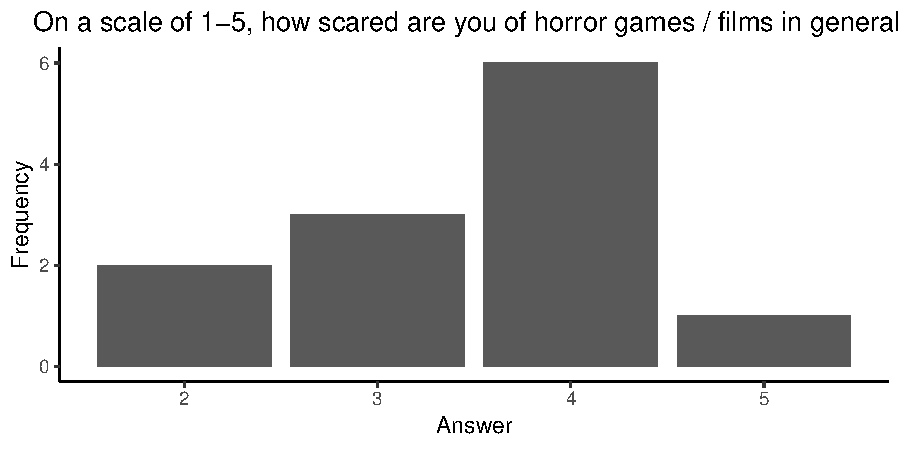
\includegraphics[width=\maxwidth]{figure/unnamed-chunk-2-1} 

}



\end{knitrout}

To control for the number of scares (so we have the same distribution of number of scares in both groups) - we run the intervention group first because the algorithm doesn't support targetting a number of scares - it depends on how the person reacts.
Then, we run the control group tests. Each person on the control group was shown the same number of scares as the person they were paired with in the previous control.

\begin{knitrout}
\definecolor{shadecolor}{rgb}{0.969, 0.969, 0.969}\color{fgcolor}

{\centering 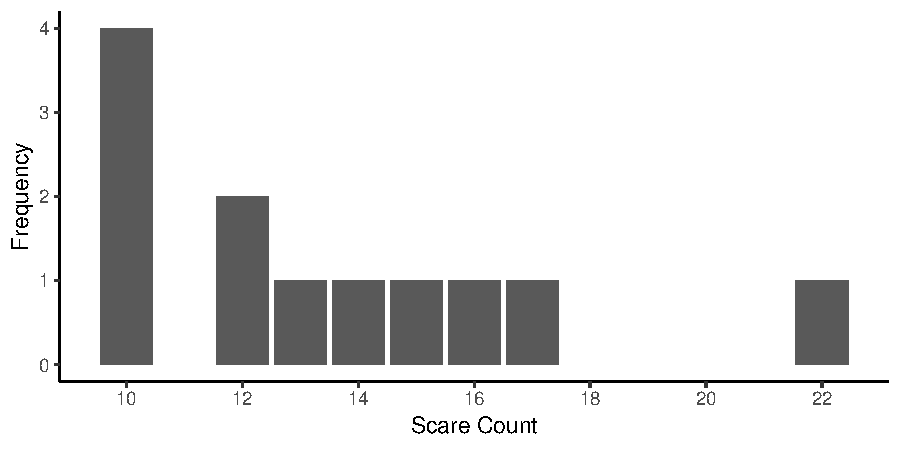
\includegraphics[width=\maxwidth]{figure/unnamed-chunk-3-1} 

}



\end{knitrout}

To control for the timing of scares - the pre-determined timings for the control group were just the timings of their intervention-group partner.
This means that for each pair that was paired up in that first control, they were shown the same number of scares at exactly the same timings, the difference being that the timings were based on the intervention-group participant's response, and not the control group participants.

Some threats to the validity of the study were present:

Frstly, the majority of the participants were young, male, and many of them were computer scientists.
I did not collect demographic data, to protect the anonymity of my participants, therefore don't have hard number, but the categories male, 18-25, and computer scientist were all in the majority.
Also, the experimental setting changed frequently.
Some tests were performed in the computer science department, which contains many other people and many distractions, while other tests were performed in quiet, private areas.
Additionally, some tests were performed at social events, meaning that participants had been drinking alcohol - though no participant was noticeably drunk.
These factors were not recorded and therefore we cannot investigate any correlation between the environmental/demographic factors and results.
While I don't believe that these threats completely invalidate the study, it does mean that any marginal results should be used only to direct further research as opposed to being taken as gosepl.

I originally aimsed to get 50 participants. Due to practical sisues, onyl 26 participants were tested. Of those, 2 participants were excluded from analysis as their EDA went too low and the sensor stopped working. Of the remaining 24 participants, 12 were allocated to each group. After 21 participants, easter break was arriving and people would start to leave durham, so I wouldn't be able to test more. At that point I started looking only for people to be the control-group participant in the pairs that only had intervention group participants. I was careful not to let people know what number they had to say to the scaredness questionto be accepted.

Attrition threat - when the risk of people dropping out / being excluded is a function of the dependent variable. This risk is present in two ways. If people are very scared, their EDA will drop more (dependent variable), and those people will also be more likely to drop out. Therefore if one group is much scarier the result won't show as clearly as some will drop out over being too scared. This risk did not occur as nobody dropped out once starting. 2 people were excluded though, and they were excluded as a direct result of their EDA. If that was as a result of their EDA dropping a lot, that would be a risk. In our case, it was due to their natural EDA being very low, with one participant remarking even before any issues occured that they had notoriously sweaty hands. I think the attrition threats are minimal.

Maturation threat - When the dependent variable is a function of time and there is a difference in time between the testing of the two groups. Since in each pair the intervention group participant is tested first, the intervention group tests on average happened before the control group tests. However, I doubt the dependent variable is a function of time - I don't think that people are any more or less scared of horror games from one week to the next and there were no newsworthy events that could have heightened people's sense of fear or anything like that.

The experiment was single-blind, in that I knew which group people were in but thy did not. There is limited researcher participation in the experiemnt so i doubt this has much of an effect. I just explained the test to them then set it going and everything happened passively.

The participants were not assigned to the groups randomly. They were assigned chronologically. As and when participants were avaialble to be gtested, they were asked for their scaredness and either placed in the control group and matched with an intervention group person or were placed int he intervention group and matched with a control group person later. Originally I planned to sample participants randomly by gettining and inition expression of interest and a 1-5 scaredness rating then assigninggroup and performing tests, but that was infeasible due to atrition rates and the general flakiness of students.

Other factors that could have ha dan effect and weren't controlled for:
Some people had played minecraft before, those that hadn't may have been more stressed. This was minimised by removing the chance of death, and giving detailed instructions and a constrained enviornment. The game was simple to learn and nobody showed any issues past the first 30 seconds or so.
Some people are more competitive when trying to collect the wool. This could have been stressful for them. This was not controlled for but there should not be any competitiveness bias between groups

There is a slim chance of intentional data vandalism. Participats could lie about how scared they were, but if we plot a scatter graph we don't see any evidence of this. %TODO scatter graph - scaredness on x, drop size on y, coloured per participant
People could inteitonally move the mouse loads, but that would have been really obvious.
People can train themselves to change their EDA at will, usually done to learn to beat a lie-detector test. That would be hard to detect, by design, but nobody showed any knowledge of EDA or GSR> It's hard to rule this out but it's a very niche skill and the chance of someone having that skill and inteitonally vandalising the data is very slim.

Since the intervention group participants were ing eneral found earlier thant he control group participants, they are more likely to be closer to me as I started by asking my friends. That was pretty shit, but give me a break. Don't @ me. This probably has no effect.

Data is probably not generalisable to the population of all people - far too many threats. However, can be used to direct further study.
Not clear whether a 10-minute test would generalise to a multi-hour play session, but was forced to limit test length for practical reasons.
Not clear whether a simple game based in minecraft where all jump-scares are the same would generalise t o a more complex game, but needed to control as much about the scare as possible.

Ethics:
Consent was gathered and participants were asked to sign consent forms.
Harm was prevented by allowing participants to ask questions, see the jump-scare, and drop out freely.
Confidentiality was achieved by using participant IDs and only linking ID to name in the consent forms, which were securely destroyed after the experiment was done. Data was stored on a password-protected device and only released if the participants signed the voluntary data release (which all participants did).
Equipoise - it's unecertain whether the intervention would be effective or better/worse, and even if it is effective it's not obvious that a scarier game is better/worse.

%explain all of my charts and methods used

\begin{knitrout}
\definecolor{shadecolor}{rgb}{0.969, 0.969, 0.969}\color{fgcolor}

{\centering 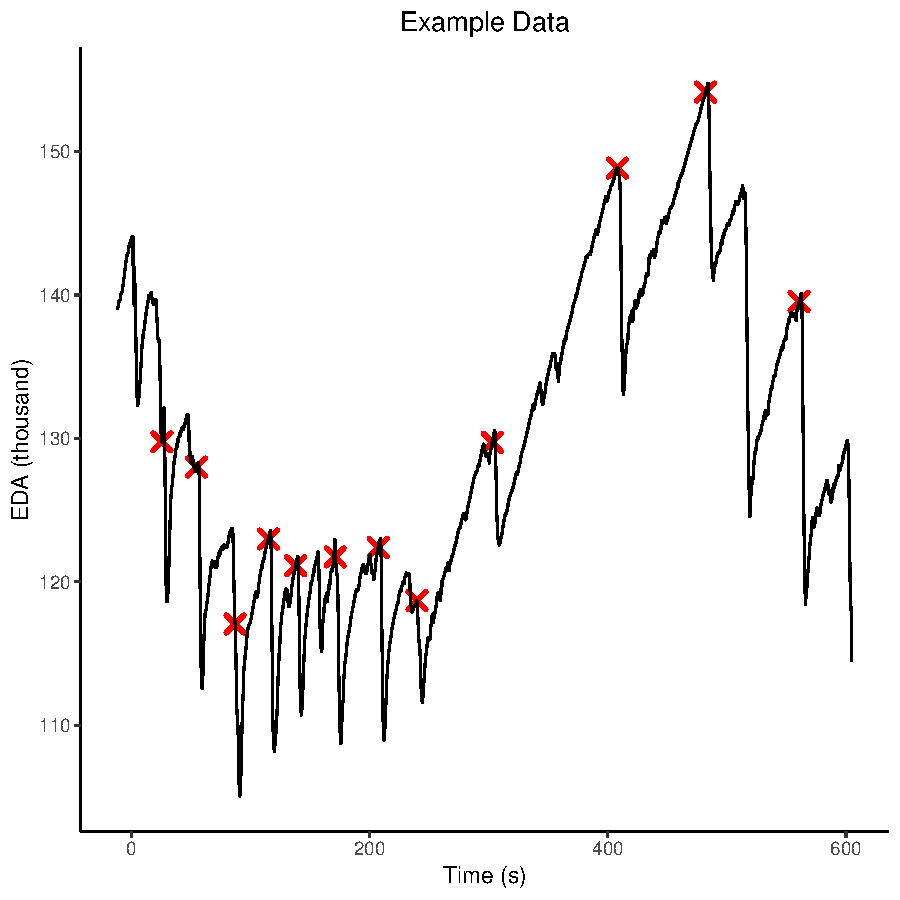
\includegraphics[width=\maxwidth]{figure/ExampleEDA-1} 

}



\end{knitrout}

\section{Results}
%Filtered jump scares that happened in the last 10 seconds

this section presents the results of the solutions.  It should include information on experimental settings.  The results should demonstrate the claimed benefits/disadvantages of the proposed solutions.

This section should be between 2 to 3 pages in length.

\section{Evaluation}

This section should between 1 to 2 pages in length.

\section{Conclusions}

This section summarises the main points of this paper.  Do not replicate the abstract as the conclusion.  A conclusion might elaborate on the importance of the work or suggest applications and extensions.  This section should be no more than 1 page in length.

The page lengths given for each section are indicative and will vary from project to project but should not exceed the upper limit.  A summary is shown in Table \ref{summary}.

\begin{table}[htb]
\centering
\caption{SUMMARY OF PAGE LENGTHS FOR SECTIONS}
\vspace*{6pt}
\label{summary}
\begin{tabular}{|ll|c|} \hline
& \multicolumn{1}{c|}{\bf Section} & {\bf Number of Pages} \\ \hline
I. & Introduction & 2--3 \\ \hline
II. & Related Work & 2--3 \\ \hline
III. & Solution & 4--7 \\ \hline
IV. & Results & 2--3 \\ \hline
V. & Evaluation & 1-2 \\ \hline
VI. & Conclusions & 1 \\ \hline
\end{tabular}
\end{table}


\bibliography{projectpaper}


\end{document}
